\chapter{Design Consideration}
In this chapter the system will be designed with a top-down approach. First a use-case of the overall functionalities in the system is described, in order to give an overall view of what the system must be able to do. Furthermore ..  

\section{Use case design}
To give an overall view of what the system should be able to do, a UML use-case diagram is used to consider and describe the main functionalities and operators in the system, see \figref{fig:usecase}.

 \begin{figure}[H]
	\centering
	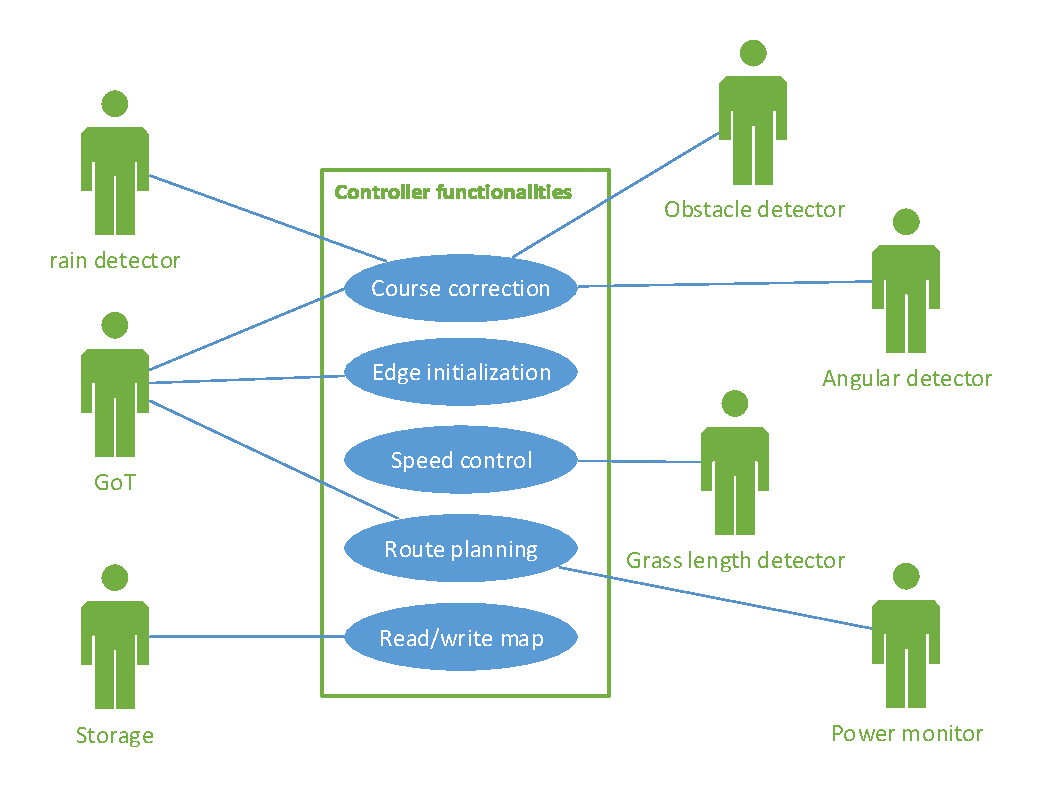
\includegraphics[scale=0.9]{figures/P5UseCase.pdf}
	\caption{Use-Case Diagram}
	\label{fig:usecase}
	\flushleft
\end{figure}

\noindent
The main purpose of the system is to automatically navigate in a specific area. In which area to navigate is decided by the \textit{Edge initialization} functionality, which uses the \textit{Store map} functionality to store the information in storage.\\\\
The route to navigate, in the specific area, is provided by the functionality \textit{Route planning}. \textit{Route planning} uses the information, about the specific area, provided by \textit{Edge initialization} to plan the most optimal route in which to follow. Furthermore the \textit{Route planning} needs information about the systems power level to insure the \textit{Route planning} takes into consideration if the system needs charging.\\\\
To insure the system is moving with a constant speed or a speed which is fitted to the height of the grass, detected with the \textit{Grass length detector}, a \textit{Speed control} functionality is necessary in the system.\\\\
The last functionality, \textit{Course correction},  
include rain sensor
the course correction is the brain speed control is the muscles. 

 


 
 